\chapter{Fundamentals}

\section{Pose Estimation}
\begin{itemize}
    \item Regression-based
    \item Heatmaps
    \item sometimes joints, sometimes body parts
\end{itemize}

\section{Human Action Recognition}

\subsection{Video-based HAR}

\subsection{Action Granularity}

\section{Neural Networks}
% TODO: Short section about motivation by biology

\subsection{Artificial Neural Networks}

\subsubsection{McCulloch-Pitts-Neuron}
One early approach inspired by the human neuron was proposed by Warren McCulloch and Walter Pitts in 1943.
The McCulloch-Pitts-Neuron (MCP), also referred to as the McCulloch-Pitts unit, takes binary input values $\bm{x} = (x_1, \dots, x_n) \in \mathbb{B}^n$ and computes a binary value $f(x_1, \dots, x_n)$.
Additionaly, the neuron itself contains a threshold value $\theta \in \mathbb{N}$.
After adding all input signals, the sum (also referred to as \textit{excitation}) is compared to $\theta$ \eref{eq:mcculloch-binary}.
%The function computing the sum is also referred to as the units \textit{excitation function} $\psi: \mathbb{B}^n \to \mathbb{N}$ while the function which evaluates the excitatin is referred to as the \textit{activation function} $\phi: \mathbb{N} \times \mathbb{N} \to \{0,1\}$.

\begin{equation}
    \begin{split}
        \label{eq:mcculloch-binary}
        f(\bm{x}, \theta) 
        &= 
        \begin{cases}
            1 & \text{if } \sum_{i=0}^n x_i \geq \theta \\
            0 & \text{otherwise}
        \end{cases}
%        \\
%        &= \phi(\psi(\bm{x}), \theta)
    \end{split}
\end{equation}

Even this simple neuron is capable of realizing some binary operators by choosing different values for $\theta$.
For example, the \textbf{boolean OR} operator is realized by setting $\theta = 1$ and the \textbf{boolean AND} operator can be achieved by choosing $\theta = n$.

A geometrical explanation of the MCP is that it separates its input space into two half-spaces, assigning the output $1$ to all input combinations on one side and $0$ on the other.
For example, for two dimensional input spaces (two input variables $x_1$ and $x_2$) this means that a MCP defines a separating line while for three dimensional input spaces the MCP becomes a separating hyperplane.
A visualization for the \textbf{boolean OR} function with three input variables is shown in \fref{fig:mcp-geometric-or}

\begin{figure}[htb!]
    \centering
    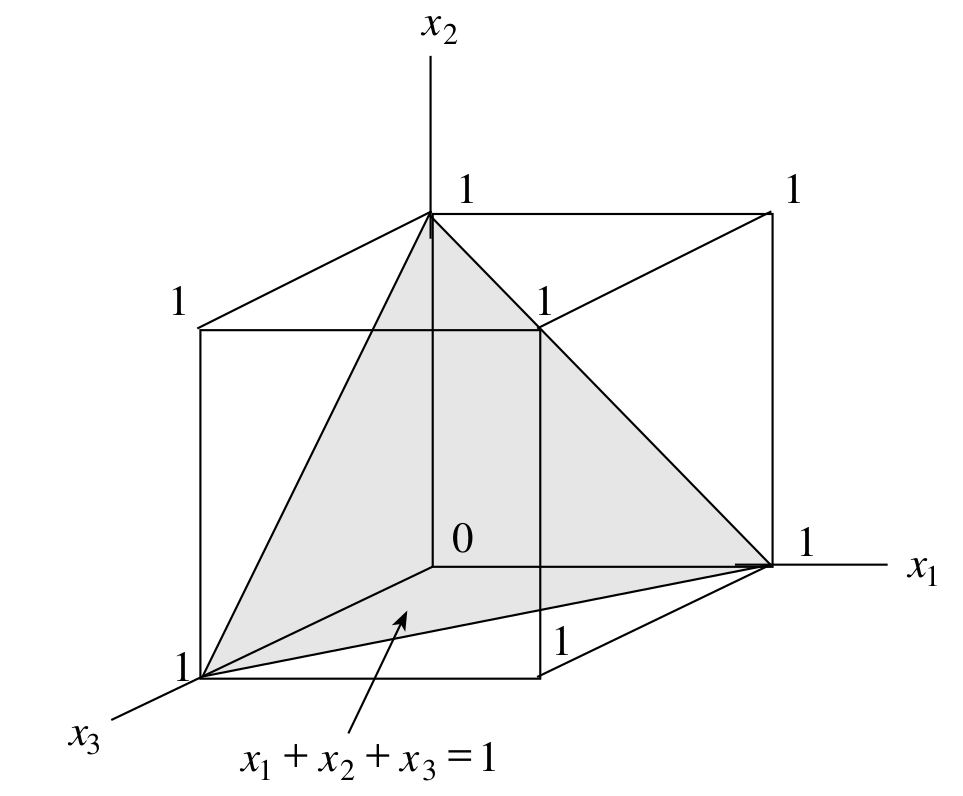
\includegraphics[width=0.6\textwidth]{mcp-geometric-or.png}
    \caption{Example of MCP dividing the three-dimensional input space using a hyperplane. The MCP is configured to model the \textbf{boolean OR} function. \cite{rojas_neural_1996}}
    \label{fig:mcp-geometric-or}
\end{figure}

The MCP looked at so far is also called an \textit{uninhibited} MCP.
\cite{rojas_neural_1996} show that \textit{uninhibited} MCP's can only model monotonic logical functions.
By adding \textit{inhibitory inputs} $\bm{y} = (y_1, \dots, y_m) \in \mathbb{B}^m$ to the MCP, however, non-monotonic logical functions like \textbf{boolean NOT} can be implemented.
The output of the MCP changes to 

\begin{equation}
    \hat{f}(\bm{x}, \bm{y}, \theta) = f(\bm{x}, \theta) \cdot \prod_{j = 0}^m (1 - y_j)
\end{equation}

Because of this definition it is possible to incorporate negated input values into the unit, giving it the ability to model a combination of negated and non-negated inputs aggregated with the \textbf{boolean AND} operator.
For example, modeling the boolean function $x_1 \wedge \neg x_2 \wedge x_3$ results to 

\begin{equation}
    \hat{f}(x_1, x_2, x_3, \theta=1) = f(x_1, x_3, \theta=1) \cdot (1 - x_2)
\end{equation}

By using two layers of units where the first layer models conjunctions just as presented above and the second layer models a simple \textbf{boolean OR} function over the outputs of the first layer it is possible to model any boolean function $f: \mathbb{B}^n \to \mathbb{B}$ because any such function can be represented in disjunctive normal form.

The obvious limitation of McCulloch-Pitts-Networks is that they are limited to the domain of logical functions.
Additionaly, they have to be constructed rather than being able to learn an approximation of the desired function because they rely on fixed connections.

% weighted vs unweighted. MCP can model this but then fixed architecture
% also: weights can thus not be learned because part of architecture (no free parameters). Want to learn these parameters. Thus: perceptron


\subsubsection{Perceptron}

In contrast to the McCulloch-Pitts-Neuron a Perceptron uses real valued inputs $\bm{x} = (x_1, \dots, x_n) \in \mathbb{R}^n$ as well as real valued weights $\bm{w} = (w_1, \dots, w_n) \in \mathbb{R}^n$ for each edge.

\begin{equation}
    f(\bm{x}, \bm{w}, \theta) = 
    \begin{cases}
        1 & \text{if } \sum_{i=0}^n w_i \cdot x_i \geq \theta \\
        0 & \text{otherwise}
    \end{cases}    
\end{equation}

Instead of setting $\theta$ as part of the neuron it is prefered to treat it as an additional trainable parameter.
To achieve this, a new fixed input value $x_b = 1$ with the corresponding weight $w_b = -\theta$ is added to the model and the previously \emph{internal} $\theta$ is fixed to $0$ \eref{eq:full-perceptron}.
This additional weight is called the \textit{bias} of the perceptron.

\begin{equation}
    \label{eq:full-perceptron}
    f(\bm{x}, \bm{w}) = 
    \begin{cases}
        1 & \text{if } ~ -w_b + \sum_{i=0}^n w_i \cdot x_i \geq 0 \\
        0 & \text{otherwise}
    \end{cases}    
\end{equation}

For notational convenience, from now on the bias is assumed to be part of $\bm{w}$, i.e. $\bm{w} = (w_1, \dots, w_n, -\theta)$ and the additional input $x_b = 1$ is part of $\bm{x}$, i.e. $\bm{x} = (x_1, \dots, x_n, -1)$.

The \textit{excitation} of a perceptron is still just a (weighted) linear combination.
This means that the perceptron, like the MCP, separates the input space by a hyperplane.
In \fref{fig:perceptron-logic} examples for some common logical functions for two input variables are provided.

\begin{figure}[htb!]
    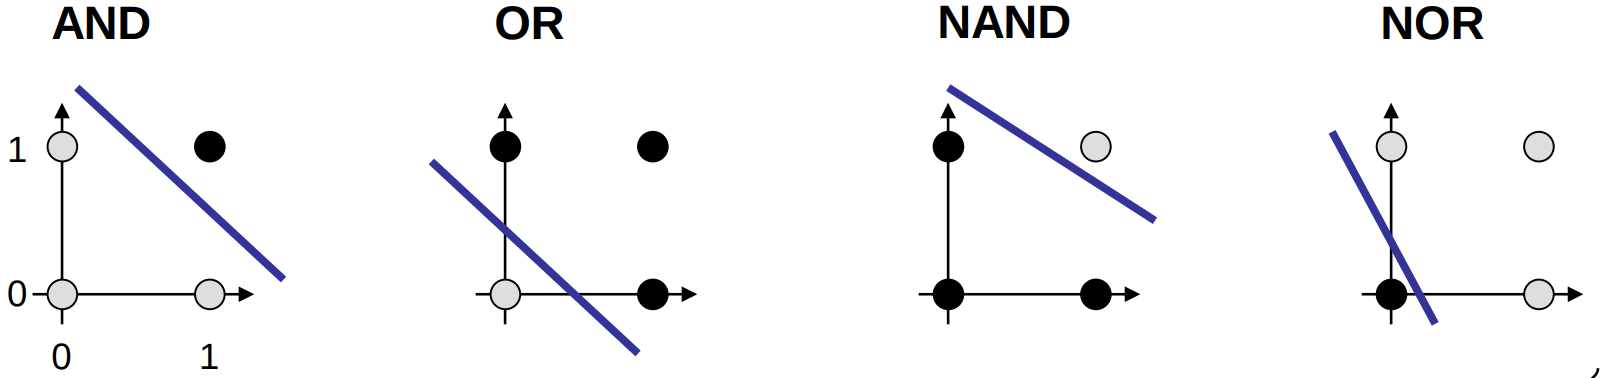
\includegraphics[width=0.9\textwidth]{perceptron-linear-seperable.png}
    \caption{Logical functions modelled by a single perceptron. The blue line indicates where the input space is divided. All input combinations on one side of the line are going to be assigned to $1$ while being assigned to $0$ on the other side. Notice that there are infinitely many possibilites for dividing lines since the input space is real valued \cite{rudolph_lecture_2018}}
    \label{fig:perceptron-logic}
\end{figure}

While MCP's were designed to model logical functions like \textbf{boolean OR} or \textbf{boolean AND} by setting $\theta$ as well as categorizing the input variables as either \textit{inhibitory} or \textit{non-inhibitory} perceptrons are able to infer these parameters by themselves through a \textit{learning process}.

Learning in the context of perceptrons means determining a parameter vector $\bm{w}$ which satisfies the following inequalities for all \textbf{positive points} $\bm{p} \in \bm{P}$ with $\hat{f}(\bm{p}, w) = 1$ as well as all \textbf{negative points} $\bm{n} \in \bm{N}$ with $\hat{f}(\bm{n}, w) = 0$

\begin{equation}
    \bm{w} \cdot \bm{p} \geq 0
\end{equation}

\begin{equation}
    \bm{w} \cdot \bm{n} < 0
\end{equation}

A parameter vector which satisfies these inequalities then defines the hyperplane separating the positive from the negative points.

The general algorithmic approach for perceptron learning is the following:
\begin{enumerate}
    \item Start with a random weight vector $\bm{w}$
    \item Evaluate how accurate the hyperplane defined by $\bm{w}$ separates the input space
    \item If positive and negative points are separated correctly:
    \begin{enumerate}
        \item Done
    \end{enumerate}
    \item Else
    \begin{enumerate}
        \item Update weight vector in a way which further reduces the error function 
        \item Go to step 2
    \end{enumerate}
\end{enumerate}

In order for the learning algorithm to determine the accuracy of a given weight vector $\bm{w}_i$ an \textbf{error function} needs to be provided.
Such a function takes all positive and negative points and calculates the amount of error (i.e. number of wrongfully classified points).
One example of an error function for binary functions is presented in \eref{eq:error-binary}\cite{rojas_neural_1996}.

\begin{equation}
    \label{eq:error-binary}
    E(\bm{w}_i) = \sum_{\bm{x} \in P} (1 - \hat{f}(\bm{x},\bm{w_i})) + \sum_{\bm{x} \in N} \hat{f}(\bm{x},\bm{w_i})
\end{equation}

It is trivial to see that the minimum error $E(\bm{w}) = 0$ is achieved if and only if $\hat{f}(\bm{x}) = 1$ for all positive points and $\hat{f}(\bm{x}) = 0$ else.

Iteratively updating the weight vector needs a strategy that guarantees that the error will be less than it was before after updating.
There are many ways to ensure that this is the case.
One algorithm, presented in \cite{rojas_neural_1996} and simply called \textit{perceptron learning algorithm}, uses the following method.

\begin{figure}[htb!]
    \centering
    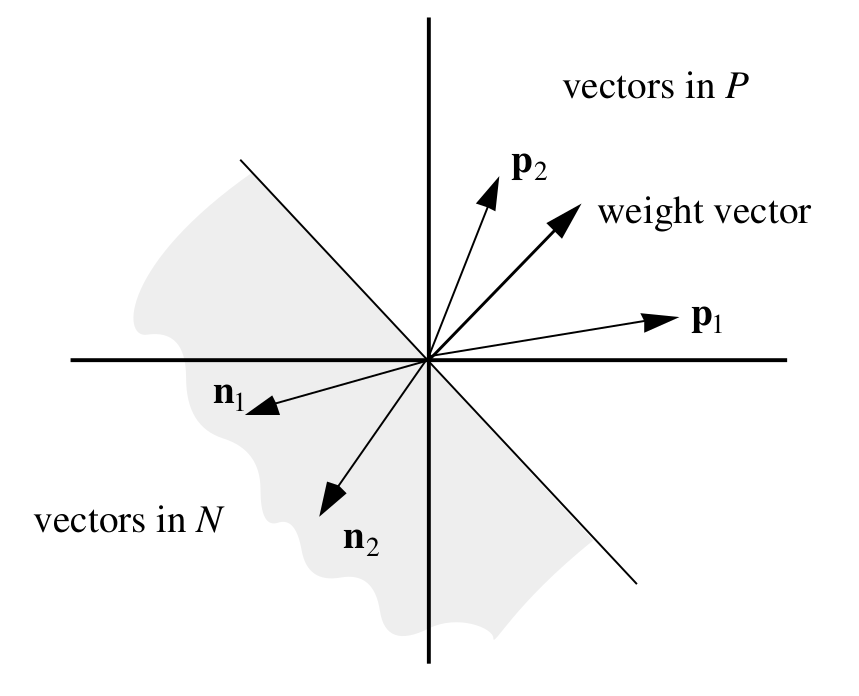
\includegraphics[width=0.55\textwidth]{perceptron-learning-update.png}
    \caption{Visualization of the weight plane $\bm{w} \cdot \bm{x}$ separating two positive and two negative vectors. The weight vector $\bm{w}$ is the normal of the hyperplane \cite{rojas_neural_1996}.}
    \label{fig:perceptron-learning-update}
\end{figure}

Given $M = P \cup N$, a point $x \in M$ is chosen randomly. 
Also, as discussed before, an random weight vector $\bm{w}_t = \bm{w}_0$ is initialized.
If $x \in P$ and $\bm{w}_t x \leq 0$ then the weight vector needs to be updated.
This is done by adding $x$ to $\bm{w}_t$.
The idea is that, in the case above, the two vectors $\bm{x}$ and $\bm{w}$ must have an angle bigger than 90 degrees (see \fref{fig:perceptron-learning-update}).
By rotating $\bm{w}$ towards $\bm{x}$ the angle will be reduced, eventually putting $\bm{x}$ on the correct side of the hyperplane.
In order to rotate $\bm{w}$ the algorithm proposes $\bm{w}_{t+1} = \bm{w}_{t} + \bm{x}$.
Analogously, if $x \in N$ and $\bm{w}_t x \geq 0$ the algorithm proposes $\bm{w}_{t+1} = \bm{w}_{t} - \bm{x}$.
This is done for each $x \in M$ where $x$ is chosen randomly.

Because $P$ and $N$ are linearly separable and there are a finite number of points it can be proven that, after a finite amount of steps, the error will be reduced to zero and the hyperplane will correctly separate the two sets.

% TODO: Maybe pocket algorithm? gives best result for when the set is not linearly seperable

\subsubsection{Gradient Descent Learning}
\textbf{TODO}
\begin{itemize}
    \item Activation functions
    \item Losses
\end{itemize}

Another approach to learning the weights of a perceptron is \textit{gradient descent}.
Given an error function $E$ with a set of initial weights $\bm{w_t}$ and an input point $\bm{x}$ the amount of error is given by $E(\bm{x}, \bm{x})$.
If the error function is differentiable one can calculate the gradient of the error function for each weight $w_i \in \bm{w}$ using 

\begin{equation}
    \frac{\partial E}{\partial w_i}
\end{equation}

which gives the direction of change which can be applied to $w_i$ in order to minimize the error function.

Consider the error function defined earlier in \eref{eq:error-binary}.
The parital derivative given each $w_i \in \bm{w}$ is then given by

\begin{equation}
    \label{eq:error-derivative-1}
    \begin{split}
        \frac{\partial E(P \cup N, \bm{w})}{\partial w_i}
        &= \frac{\partial }{\partial w_i} \sum_{x \in P} (1 - \hat{f}(\bm{x},\bm{w_i})) + \sum_{\bm{z} \in N} \hat{f}(\bm{z},\bm{w_i}) \\
        &= \frac{\partial }{\partial w_i} \sum_{x \in P} (1 - \hat{f}(\bm{x},\bm{w_i})) + \frac{\partial }{\partial w_i} \sum_{\bm{z} \in N} \hat{f}(\bm{z},\bm{w_i}) \\
        &= \sum_{x \in P} \frac{\partial }{\partial w_i} (1 - \hat{f}(\bm{x},\bm{w_i})) + \sum_{\bm{z} \in N} \frac{\partial }{\partial w_i} \hat{f}(\bm{z},\bm{w_i}) \\
        &= \sum_{x \in P} - \frac{\partial }{\partial w_i} \hat{f}(\bm{x},\bm{w_i}) + \sum_{\bm{z} \in N} \frac{\partial }{\partial w_i} \hat{f}(\bm{z},\bm{w_i}) 
    \end{split}
\end{equation}

This presents a challange, however.
Until now, the formal definition of a single perceptron was 

\begin{equation}
    \begin{split}
        \hat{f}(\bm{x}, \bm{w}) 
        &=         
            \begin{cases}
                1 & \text{if } \bm{w} \cdot \bm{x} \geq 0 \\
                0 & \text{otherwise}
            \end{cases} 
        \\
        &= \phi(\bm{x} \cdot \bm{w})
        \\
        &= \phi(\psi(\bm{x}, \bm{w}))
    \end{split}
\end{equation}

where $\psi$ is called the \textit{integration function} which computes the excitation and $\phi$ the \textit{activation function} which computes the activation of the neuron.

This results in a non-differentiable activation function since the thresholding approach is not continuous, it cannot be differentiable either.
A popular choice for a differentiable activation function is the \textit{sigmoid activation function} $S(x)$ given by

\begin{equation}
    S(x) = \frac{1}{1 + e^{-x}}
\end{equation}

One can easily see that the sigmoid function is differentiable and that the derivative is given by 

\begin{equation}
    \begin{split}
        \frac{d}{dx} S(x) 
        &= \frac{e^{-x}}{(1 + (e^{-x})^2)} \\
        &= S(x)(1 - S(x)) 
    \end{split}
\end{equation}

By then choosing $\phi = S$ and keeping $\psi(\bm{x}, \bm{w}) = \bm{x} \cdot \bm{w}$ in \eref{eq:error-derivative-1} the partial derivative of the error function becomes

\begin{equation}
    \label{eq:error-derivative-2}
    \begin{split}
        \frac{\partial E(P \cup N, \bm{w})}{\partial w_i}
        &= \sum_{x \in P} - \frac{\partial }{\partial w_i} \hat{f}(\bm{x},\bm{w_i}) + \sum_{\bm{z} \in N} \frac{\partial }{\partial w_i} \hat{f}(\bm{z},\bm{w_i})  \\
        &=  \sum_{x \in P} - \frac{\partial }{\partial w_i} \psi(\phi(\bm{x},\bm{w_i})) + \sum_{\bm{z} \in N} \frac{\partial }{\partial w_i} \psi(\phi(\bm{z},\bm{w_i})) \\
        &=  - \sum_{x \in P} \frac{\partial }{\partial w_i} S(\bm{x} \cdot \bm{w_i}) + \sum_{\bm{z} \in N} \frac{\partial }{\partial w_i} S(\bm{z} \cdot \bm{w_i}) \\
        &=  - \sum_{x \in P}  S(\bm{x} \cdot \bm{w_i}) (1 - S(\bm{x} \cdot \bm{w_i})) + \sum_{\bm{z} \in N} S(\bm{z} \cdot \bm{w_i}) (1 - S(\bm{z} \cdot \bm{w_i}))\\
    \end{split}
\end{equation}

After computing the partial derivative for each $w_i \in \bm{w}$ the \textit{gradient} then is 

\begin{equation}
    \nabla E(P \cup N, \bm{w}) = \left(\frac{\partial E(P \cup N, \bm{w})}{\partial w_1}, \dots, \frac{\partial E(P \cup N, \bm{w})}{\partial w_n} \right)
\end{equation}

Finally, the current weights $\bm{w_t}$ can be updated by changing the weights a certain \textit{step size or learning rate} $\gamma$ towards a local minimum of the error function by applying 

\begin{equation}
    \label{eq:gradient-binary-update}
    \bm{w_{t+1}} = \bm{w_t} - \gamma \nabla E(P \cup N, \bm{w_t})
\end{equation}

Since the gradient points toward the steepest ascent of the error function a negation is needed to approach the local minimum.

In the literature, the terms \textit{error function} and \textit{loss function} are sometimes used interchangeably.

\subsubsection{Multi-Layer Perceptron}
Until now, the assumption was made that the two sets of points $P$ and $N$ are linearly separable.
Many problems, however, are more complex and cannot be easily separated linearly.
One example from the realm of logical functions is the \textbf{XOR} function.
As an example, consider \textbf{XOR} with two input variables.
If visualized in the same way as in \fref{fig:perceptron-logic} it is quite trivial to see that no single line is able to divide the positive from the negative points.
Therefor, a more complex model is necessary for modeling functions with \textit{convex solution spaces} such as \textbf{XOR} \fref{fig:xor-convex}.
One way of incorporating more complexity is by grouping perceptrons into \textit{layers} and connecting them together.

\begin{figure}[htb!]
    \centering
    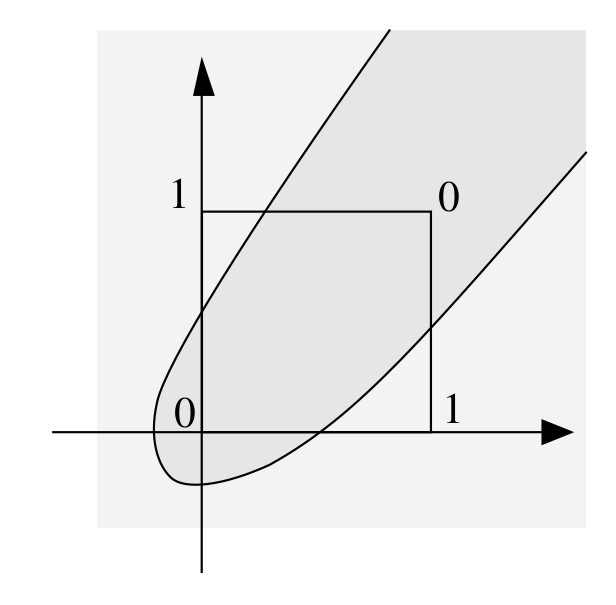
\includegraphics[width=0.5\textwidth]{xor-convex.png}
    \caption{Solving the \textbf{XOR} problem by using separating \textit{regions} instead of hyperplanes \cite{rojas_neural_1996}}
    \label{fig:xor-convex}
\end{figure}

Let $\bm{N} = (N_1, \dots, N_L)$ be a \textit{multi-layer perceptron (MLP)} consisting of $L$ layers.
In the literature, the inputs are also considered a layer, even though they do not consist of perceptrons.
This then means that a MLP has one input layer, several \textit{hidden layer} with the last hidden layer also providing the output.
When reffering to the number of layers of a MLP only the hidden layer are counted, meaning that a MLP consisting of $L=3$ layer has one input layer and three hidden layer.

Each hidden layer $N_l$ consists of $m_l \in \mathbb{N}$ perceptrons.
Consecutive layers are connected by directed, weighted edges $w_{ij} \in \mathbb{R}$ with $n_i \in N_l$ and $n_j \in N_{l+1}$ so that each perceptron $n_i$ is connected to the input of each perceptron $n_j$ in the consecutive layer.
Two perceptrons inside the same layer are not allowed to be connected in traditional MLP definitions.
Also, the inputs to the MLP are only allowed to be connected to the first layer $N_1$.

%The name \textit{multi-layer perceptron} is often used interchangeably to \textit{artificial neural network} which is why, from now on, both will refer to the same concept.

By choosing $L=2$ a MLP is capable of modeling every convex solution space \cite{rojas_neural_1996}.
The perceptrons in the first layer each learn to linearly separate the solution space into two parts like described earlier.
By using just one perceptron in the second layer this perceptron is able to learn the \textbf{boolean AND} function over all outputs from the first layer.
This means that it is possible to learn a convex solution space similar to \fref{fig:convex-solution}.

\begin{figure}[htb!]
    \centering
    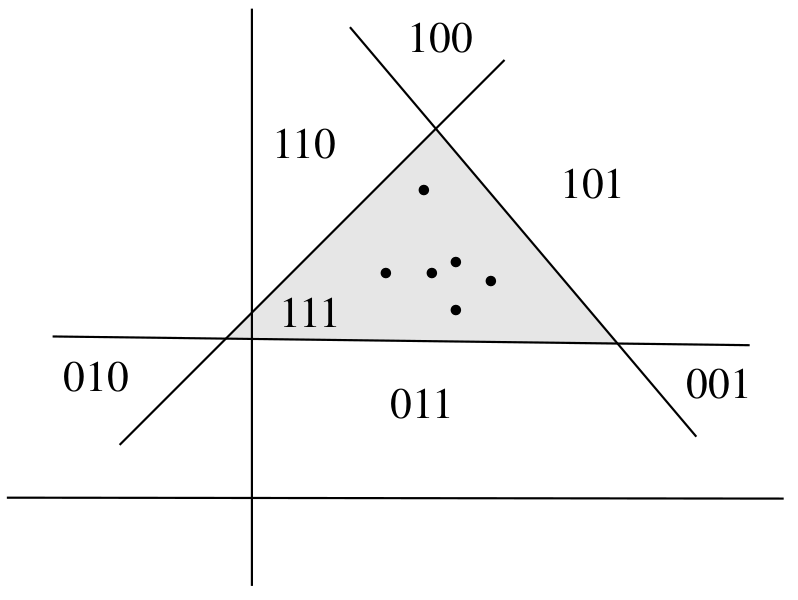
\includegraphics[width=0.8\textwidth]{convex_solution_space.png}
    \caption{Example of a convex solution space using a two-layered MLP with three perceptrons in the first and one perceptron in the second layer. Each bitvector $b = (x_1, x_2, _3)$ shows the output of perceptron 1, 2 and 3 respectively \cite{rojas_neural_1996}}
    \label{fig:convex-solution}
\end{figure}

Even with the ability to model every convex solution space, there are still problems which have a \textit{non-convex solution space}.
However, by adding another layer to the MLP ($L=3$) these problems can be solved.

The first hidden layer behaves just like in the previous example with each perceptron splitting the input space into two.
Each perceptron in the second layer again learns \textbf{boolean AND} functions, resulting in $\lVert N_2 \rVert$ regions.
In the third layer, a perceptron then combines these regions into non-convex regions using the learned \textbf{boolean OR} operator.
In fact, a three-layer MLP is able to model any arbitrary function (with enough perceptrons per layer).

These intuitive ideas of how the MLP is able to model any arbitrary function does not imply, however, that each perceptron in the third layer \textit{has} to learn the \textbf{boolean OR} function etc.
They just show that these MLPs are powerful enough to model any arbitrary function by combining simple features (separating lines) from previous layers to form new, more complex features (combinations of convex regions) with each consecutive layer.

\subsubsection{Backpropagation}

Probably the most common learning algorithm for training MLPs is the \textbf{backpropagation algorithm}, initially proposed by Paul Werbos in 1974 and popularized by Rumelhart, Hinton and Williams in 1986.
It uses gradient descent with the addition of propagating the error backwards through the network by making use of the chain rule of derivation.

For each point $\bm{x_i}$ in the training data, the algorithm follows these steps:

\begin{enumerate}
    \item Start with random weights $\bm{W}_0 = (\bm{w_{1_0}}, \dots, \bm{w_{N_0}})$ for each neuron.
    \item Pass $\bm{x_i}$ into the network (called a \textit{forward pass})
    \begin{itemize}
        \item $\hat{f}(\bm{x_i}, \bm{w}_0) = \bm{y_i}$
    \end{itemize}
    \item Compute gradient at the last layer by using a loss function and the expected result $\hat{\bm{y_i}}$.
    \item Compute gradient for the previous layers, incorporating the error from the consecutive layers (called a \textit{backward pass}).
    \item Update the weights with their corresponding gradients.
\end{enumerate}

In order to show how the backpropagation algorithm works consider a MLP with $L=2$ hidden layer $L_1, L_2$ and $\left| \bm{x} \right| = N$ inputs.
Also, let $\lVert L_1 \rVert = \lVert L_2 \rVert = M$ without loss of generality.

First, the forward pass is performed.
The output of each neuron $h_j(\bm{x}, \bm{w_j}) = y_j$ in the first hidden layer can be described using the following equation

\begin{equation}
    \begin{split}
        h_j(\bm{x}, \bm{w_j}) 
        &= S(\bm{x} \cdot \bm{w_j}) \\
        &= \frac{1}{1 + e^{-(\bm{x} \cdot \bm{w_j})}}
    \end{split}
\end{equation}

Similarly, after the second layer, the output $g_k$ for each neuron given the network input can be described as 

\begin{equation}
    \begin{split}
        g_k(\bm{x}, \bm{w_k}) 
        &= S\left(\sum_{j=0}^M w_{jk} \cdot h_j(\bm{x}, \bm{w_j})\right) \\
        &= S\left(\sum_{j=0}^M w_{jk} \cdot \left(\sum_{i=0}^N w_{ij} x_i\right)\right)
    \end{split}
\end{equation}

For notational convenience, instead of \eref{eq:error-binary}, consider the following loss function.
Every differentiable loss function can be used in the backpropagation algorithm.

\begin{equation}
    SSE(\bm{w}) = \sum_{\bm{x} \in B} (\hat{f}(\bm{x}, \bm{w}) - y_x)^2
\end{equation}

This loss function, the \textbf{sum of squared errors}, computes the output of the perceptron $\hat{f}(\bm{x}, \bm{w})$ for a given weight vector $\bm{w}$ and subtracts the expected output $y_x$ for the input $\bm{x}$.
By computing the square of the result the error value will be positve and larger errors will contribute more towards the error sum.

% TODO: Ich glaube es wurde noch nirgendwo das wort training data benutzt. Das kommt am besten schon in perceptron learning vor

After the forward pass through the network the loss for a single output neuron $g_k$ is given by

\begin{equation}
    \begin{split}
        SSE(\bm{x}, (\bm{w_j}, \bm{w_k})) 
        &= (y_k - \hat{y}_{k})^2 \\
        &= (g_k(\bm{x},\bm{w_k}) - \hat{y}_{k})^2 \\
        &= \left(S \left(\sum_{j=0}^M w_{jk} \cdot h_j(\bm{x}, \bm{w_j})\right) - \hat{y}_{k}\right)^2 \\
        &=  \left( S\left(\sum_{j=0}^M w_{jk} \cdot S \left(\sum_{i=0}^N w_{ij} x_i\right)\right) - \hat{y}_{k}\right)^2
    \end{split}
\end{equation}

By using the same approach as with gradient descent, the partial derivative of the loss function with regards to the weights of the second layer is given by 

\begin{equation}
    \begin{split}
        \frac{\partial ~ SSE(\bm{x}, \bm{w})}{\partial w_{jk}}
        &= \frac{\partial}{\partial w_{jk}} (g_k(\bm{x},\bm{w_k}) - \hat{y}_{k})^2
    \end{split}
\end{equation}

Using the chain rule for derivation 

\begin{equation}
    (p(b(x)))' = p'(b(x)) \cdot b'(x)
\end{equation}

the partial derivative can be broken down into 

\begin{equation}
    \begin{split}
        \frac{\partial ~ SSE(\bm{x}, \bm{w})}{\partial w_{jk}}
        &= \frac{\partial}{\partial w_{jk}} ~ (g_k(\bm{x},\bm{w_k}) - \hat{y}_{k})^2 \\
        &= 2 \cdot (g_k(\bm{x},\bm{w_k}) - \hat{y}_{k}) \cdot  S'\left(\sum_{j=0}^M w_{jk} \cdot h_j(\bm{x}, \bm{w_j})\right) \cdot h_j(\bm{x}, \bm{w}_j) \\
        &= 2 \cdot (y_k - \hat{y}_{k}) \cdot  y_k \cdot (1 - y_k) \cdot h_j(\bm{x}, \bm{w_j}) \\
        &= \delta_k \cdot h_j(\bm{x}, \bm{w_j}) \\
        &= \delta_k \cdot y_j
    \end{split}
\end{equation}

One can observe that the output of all neurons from layer $N_{k}$ are needed to compute the partial derivate for neurons in layer $N_{k+1}$, which is why the initial forward pass through is necessary.

Similarly, the partial derivative of the loss function with regards to $w_{ij}$ is given by \eref{eq:backprop-partial-hidden}. 
However, while running backpropagation, the partial derivatives of all nodes in layer $N_{k+1}$ need to be computed first in order to determine the partial derivative of nodes in layer $N_{k}$ \cite{rojas_neural_1996}.

\begin{equation}
    \label{eq:backprop-partial-hidden}
    \begin{split}
        \frac{\partial ~ SSE(\bm{x}, \bm{w})}{\partial w_{ij}}
        &= \frac{\partial}{\partial w_{ij}} ~ (g_k(\bm{x},\bm{w_k}) - \hat{y}_{k})^2 \\
        &= 2 \sum_{k=0}^{K} (g_k(\bm{x},\bm{w_k}) - \hat{y}_{k}) \cdot  S'\left(\sum_{j=0}^M w_{jk} \cdot h_j(\bm{x}, \bm{w_j})\right) \cdot w_{jk} \cdot S'(\bm{x} \cdot \bm{w_j}) \cdot x_i \\
        &= 2 \sum_{k=0}^{K} (g_k(\bm{x},\bm{w_k}) - \hat{y}_{k}) \cdot  g_k(\bm{x},\bm{w_k}) \cdot (1-g_k(\bm{x},\bm{w_k})) \cdot w_{jk} \cdot h_j(\bm{x}, \bm{w_j}) \cdot (1-h_j(\bm{x}, \bm{w_j})) \cdot x_i \\
        &= 2 \sum_{k=0}^{K} (y_k - \hat{y}_{k}) \cdot  y_k \cdot (1-y_k) \cdot w_{jk} \cdot y_j \cdot (1-y_j) \cdot x_i \\
        &= x_i \cdot y_j \cdot (1-y_j) \cdot \sum_{k=0}^{K} 2 \cdot (y_k - \hat{y}_{k}) \cdot y_k \cdot (1 - y_k) \cdot w_{jk} \\
        &= x_i \cdot y_j \cdot (1-y_j) \cdot \sum_{k=0}^{K} \delta_k \cdot w_{jk} \\
        &= x_i \cdot \delta_j
    \end{split}
\end{equation}

After computing all partial derivatives for all neurons in the network, the weights can be updated, similarly to \eref{eq:gradient-binary-update}, using the following formulas:

\begin{equation}
    \begin{split}
        w_{jk_{t+1}} 
        &= w_{jk_{t}}  - \gamma \cdot \frac{\partial ~ SSE(\bm{x}, \bm{w})}{\partial w_{jk}} \\
        &= w_{jk_{t}}  - \gamma \cdot \delta_k \cdot y_j
    \end{split}
\end{equation}

\begin{equation}
    \begin{split}
        w_{ij_{t+1}} 
        &= w_{ij_{t}} - \gamma \cdot \frac{\partial ~ SSE(\bm{x}, \bm{w})}{\partial w_{ij}} \\
        &= w_{ij_{t}} - \gamma \cdot \delta_j \cdot x_i
    \end{split}
\end{equation}


\subsection{Convolutional Neural Networks}
\subsubsection{Convolutional Layer}
Perceptive Field


\subsubsection{Pooling Layer}

\subsubsection{Fully-Connected Layer}